\documentclass[12pt,a4paper]{article}

\usepackage{cite}
\usepackage{natbib}
\usepackage{pifont}
\usepackage{amsmath,amsfonts,amsthm} % Math packages for equations
\usepackage[svgnames]{xcolor} % Enabling colors by their 'svgnames'
\usepackage{graphicx} % Required for adding images
\usepackage{framed}
\usepackage{tcolorbox}
\usepackage{geometry} % Required for adjusting page dimensions
\usepackage{titling}

\definecolor{ColorDef}{rgb}{0.00, 0.75, 1.00}

\geometry{
	top=1.5cm, % Top margin
	bottom=1.5cm, % Bottom margin
	left=2.5cm, % Left margin
	right=2.5cm, % Right margin
	includehead, % Include space for a header
	includefoot, % Include space for a footer
	%showframe, % Uncomment to show how the type block is set on the page
}

\renewcommand\familydefault{\sfdefault}

\pretitle{%
  \begin{center}
  Delft University of Technology (T\textcolor{ColorDef}{U} Delft)\\
  M.Sc. Thesis Proposal\\
  \vspace{5mm}
}
\posttitle{\end{center}}

\begin{document}

\title{\LARGE \textbf{Title of the Prospective Thesis}}
\date{} 

\vspace{-10mm}


\maketitle
  \vspace{-20mm}
\vspace{-0.5cm}
\textcolor{ColorDef}{\hrule}
\vspace{-0.5cm}
\section*{}
\textbf{Keywords:} Keyword 1, Keyword 2, Keyword 3, Keyword 4
\setlength{\parindent}{0cm}

\vspace{+0.25cm}
\textcolor{ColorDef}{\hrule}
\vspace{-0.5cm}
%
\section*{}
Paragraph one (preferably 3-5 lines), where you explain the main/mother field. The following figure is an example one where you can put a nice banner-like representative figure from your own field.

\vspace{+0.5cm}
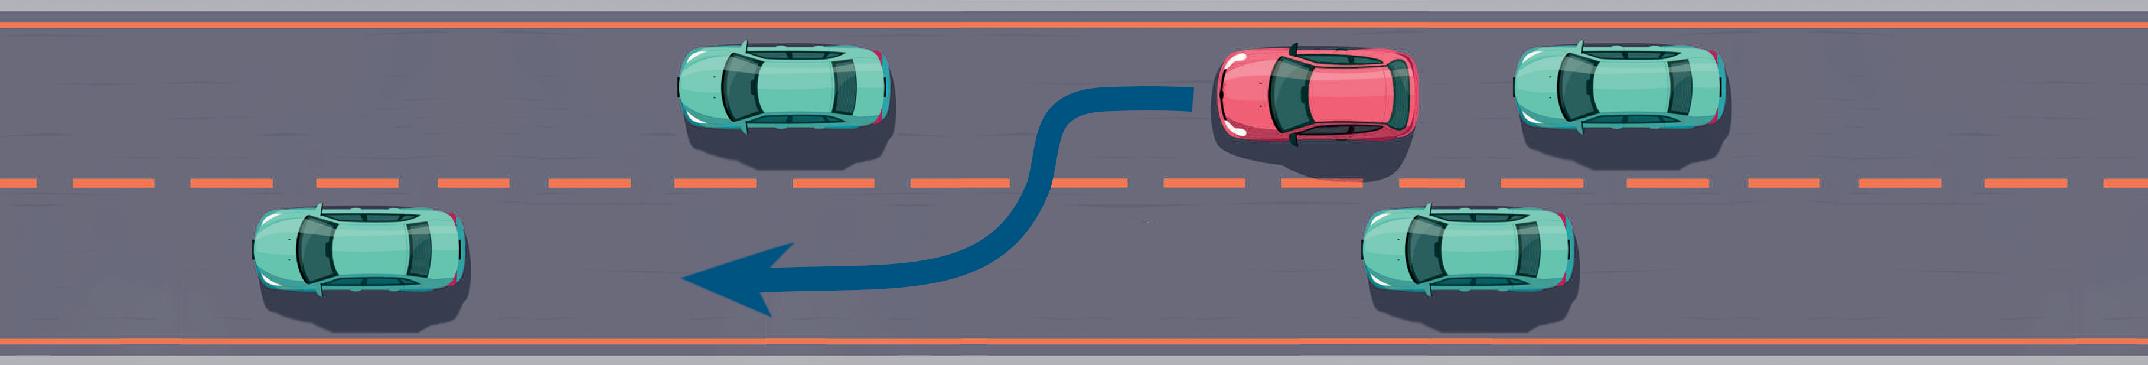
\includegraphics[width=\textwidth]{Cars.pdf}
\vspace{+0.25cm}

Paragraph two (preferably 7-10 lines), where you explain the sub-field.

\vspace{+0.5cm}
\textcolor{ColorDef}{\hrule}
\vspace{+0.75cm}

\textbf{Research plan:} \emph{Upon carefully reviewing the literature,}, ... this is where you explain what is the objective of the prospective project (preferably in 4-6 lines). \\
 
If this proposal appeals to you as an M.Sc. project, please contact us for more information. 

\vspace{+0.25cm}
\textcolor{ColorDef}{\hrule}
\vspace{+0.5cm}

\textbf{Contact persons:} \\
\hspace*{2ex} First Supervisor: \texttt{F.Supervisor@tudelft.nl}\\
\hspace*{2ex} Second Supervisor: \texttt{S.Supervisor@tudelft.nl} 

\end{document}